\newpage
\section{Results}
\subsection{The change in aerosol concentrations}
After applying the high-pressure blocking detection method to the data from Vavihill for the entire period, a total of 298 high-pressure blocking events were identified between August 1, 1995, and October 10, 2024. Of these 298 events, 155 were removed due to insufficient \PM  data, as a filter requiring 85\% data coverage was applied. This left 143 relevant high-pressure blocking events. For Malmö, a total of 299 high-pressure blocking events were identified between November 20, 1995, and October 1, 2024. From these, 77 events were removed due to insufficient \PM  data, again applying the 85\% data coverage filter. This resulted in 222 relevant high-pressure blocking events. All of the categories had a p-value approximately equal to 0. An example plot showing the periods of high-pressure blocking events can be seen in \autoref{fig:2001}.


\autoref{fig:2001} provides insight int other categorization of high-pressure blocking events for the two different locations. One can note differences in the lengths of the events. One can also note that the event during the first of February is only observed in Malmö, but not in Vavihill. The other way around can be seen during the midway through October. Since the pressure differences between the stations only differ by a few hPa, these differences indicate a difference in precipitation, as can bee seen in the figure below. 

\begin{figure}[H]
    \centering
    \begin{subfigure}[b]{0.49\textwidth}
        \centering
        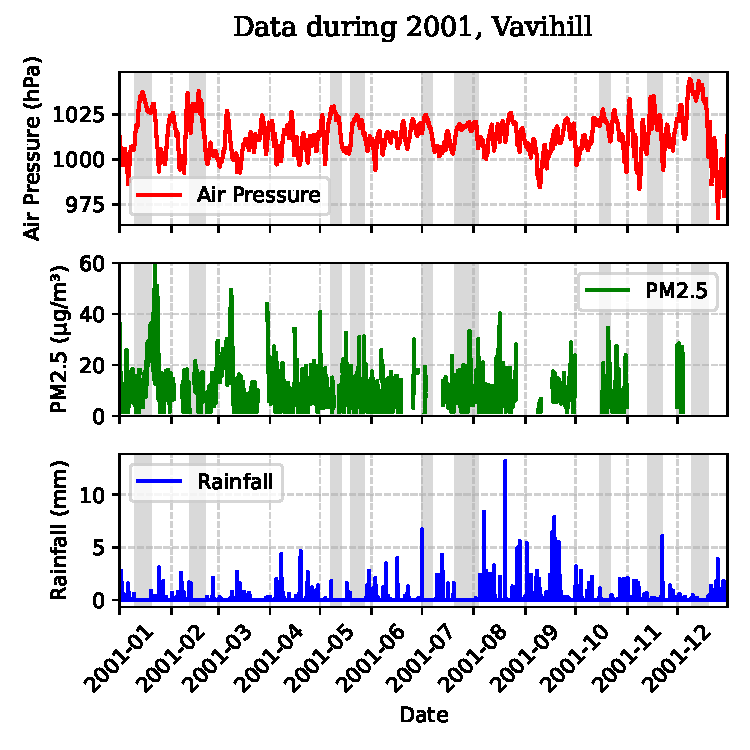
\includegraphics[width=\textwidth]{Figures/Vavihill_plot_20010101_20011231.pdf}
        \label{fig:2001Vavihill}
    \end{subfigure}
    \hfill
    \begin{subfigure}[b]{0.49\textwidth}
        \centering
        \includegraphics[width=\textwidth]{Figures/Malmö_plot_20010101_20011231.pdf}
        \label{fig:2001Malmö}
    \end{subfigure}
    \caption{These example plots displays the air pressure, \PM  concentrations, and rainfall during the year 2001. The periods which was indicated as periods of high-pressure blocking events are shown in gray. }
    \label{fig:2001}
\end{figure}

The average change in \PM concentrations during periods of high-pressure blocking can be seen in \autoref{fig:Meanplot_Comparison}. The data is compared with the \PM mean taken from periods without high-pressure blocking events. An increase in \PM concentrations can be seen in Malmö, while a slight increase can be observed in Vavihill. This is supported by the large $\tau$-value in the case of Malmö (0.85), and slight lower in Vavihill (0.68). The Sen's slope values also indicate a stronger increase in Malmö \SI{3.0e-02}{} compared too \SI{1.7e-02}{} in Vavihill. After the first five days, the number of datasets decreases, which is reflected in the increase in standard deviation.


\begin{figure}[H]
    \centering
    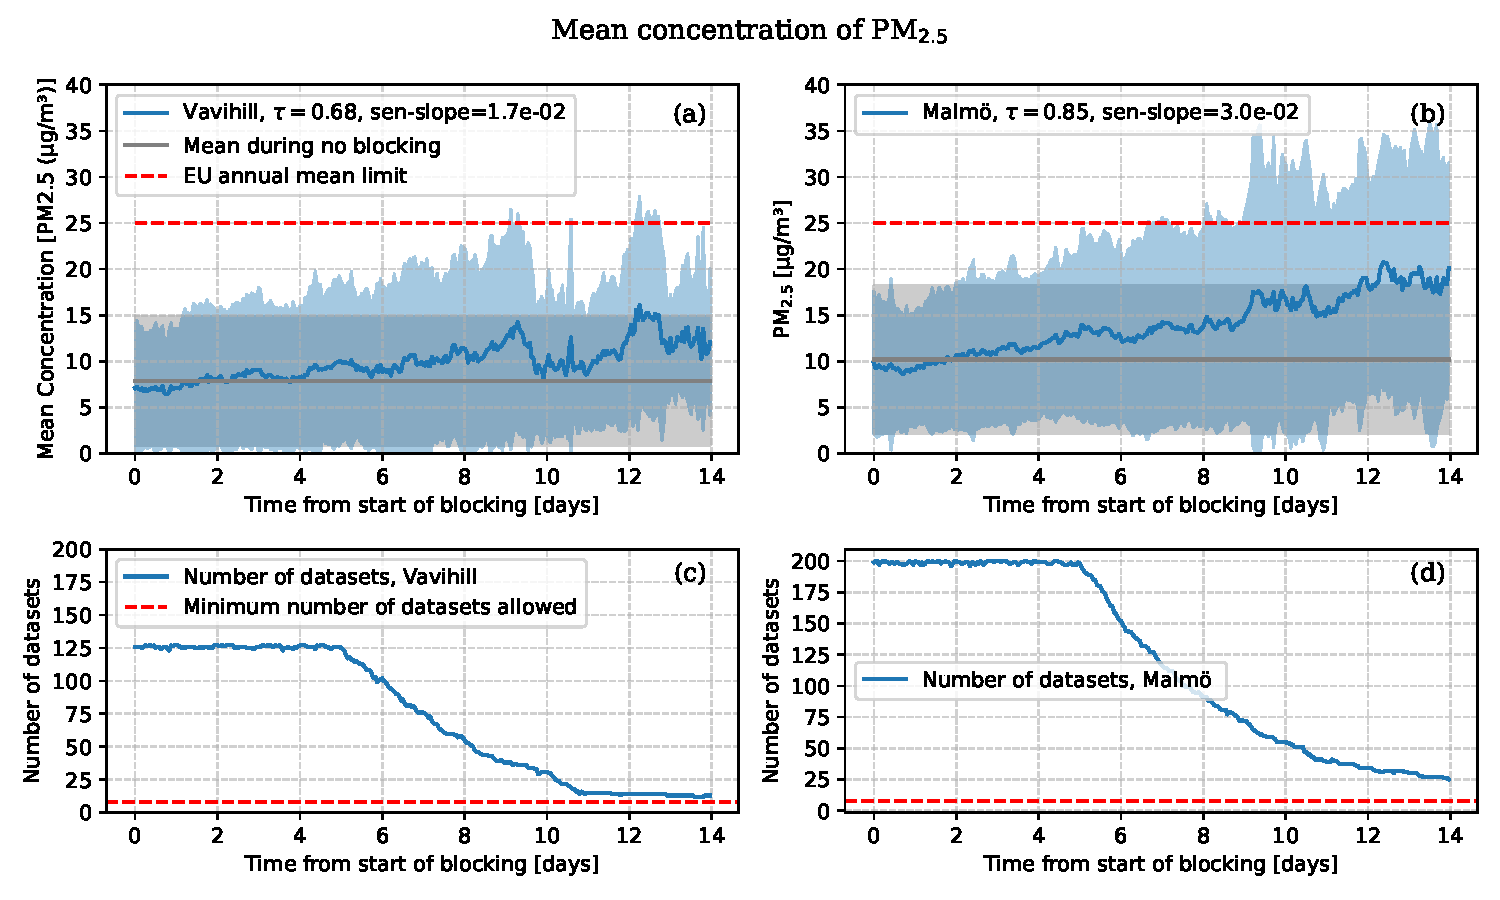
\includegraphics[width=\textwidth]{Figures/Meanplot.pdf}
    \caption{Comparison of mean \PM  concentrations in Vavihill (a) and Malmö (b), highlighting differences between rural and urban air quality. The shaded region indicates the standard deviation of the data. The number thu number of events used in the analysis can be seen in (c) and (d).}
    \label{fig:Meanplot_Comparison}
\end{figure}

\subsection{The change in aerosol concentrations depending on wind direction}

The change in \PM concentrations in Vavihill and Malmö for different wind directions can be seen in \autoref{fig:Meanplot_wind}. In the case of Vavihill, 7.0\% of the winds came from the northeast (310° to 70°), 28.0\% from the southeast (70° to 190°), 43.4\% from the west (190° to 310°) and 43.4\% from no specific direction. In the case of Malmö, 8.1\% of the winds came from the northeast (310° to 70°), 23.4\% from the southeast (70° to 190°), 18.5\% from the west (190° to 310°) and 50.0\% from no specific direction. 

One can see similarities between the aerosol concentrations depending on wind directions for Vavihill and Malmö, although a larger increase can be observed Malmö. When the wind filter was applied for the northeast direction, no strong increase or high levels of \PM  were detected, as supported by the $\tau$-values being under 0.5 for both locations. The $\tau$-value in Vavihill for southeastern directions yielded a value of 0.33. However there is a clear increase until day nine, where the levels suddenly drop. The $\tau$-value for the first nine days is 0.60, showing a clear increase. For the western wind direction, an increase in \PM can be seen in both locations as supported by the $\tau$-values (0.60 for Vavihill and 0.68 för Malmö). Elevated levels can be seen in Malmö for the west direction, and especially the southeastern direction where the mean concentration exceeds the EU annual mean limit. 

\begin{figure}[H]
    \centering
    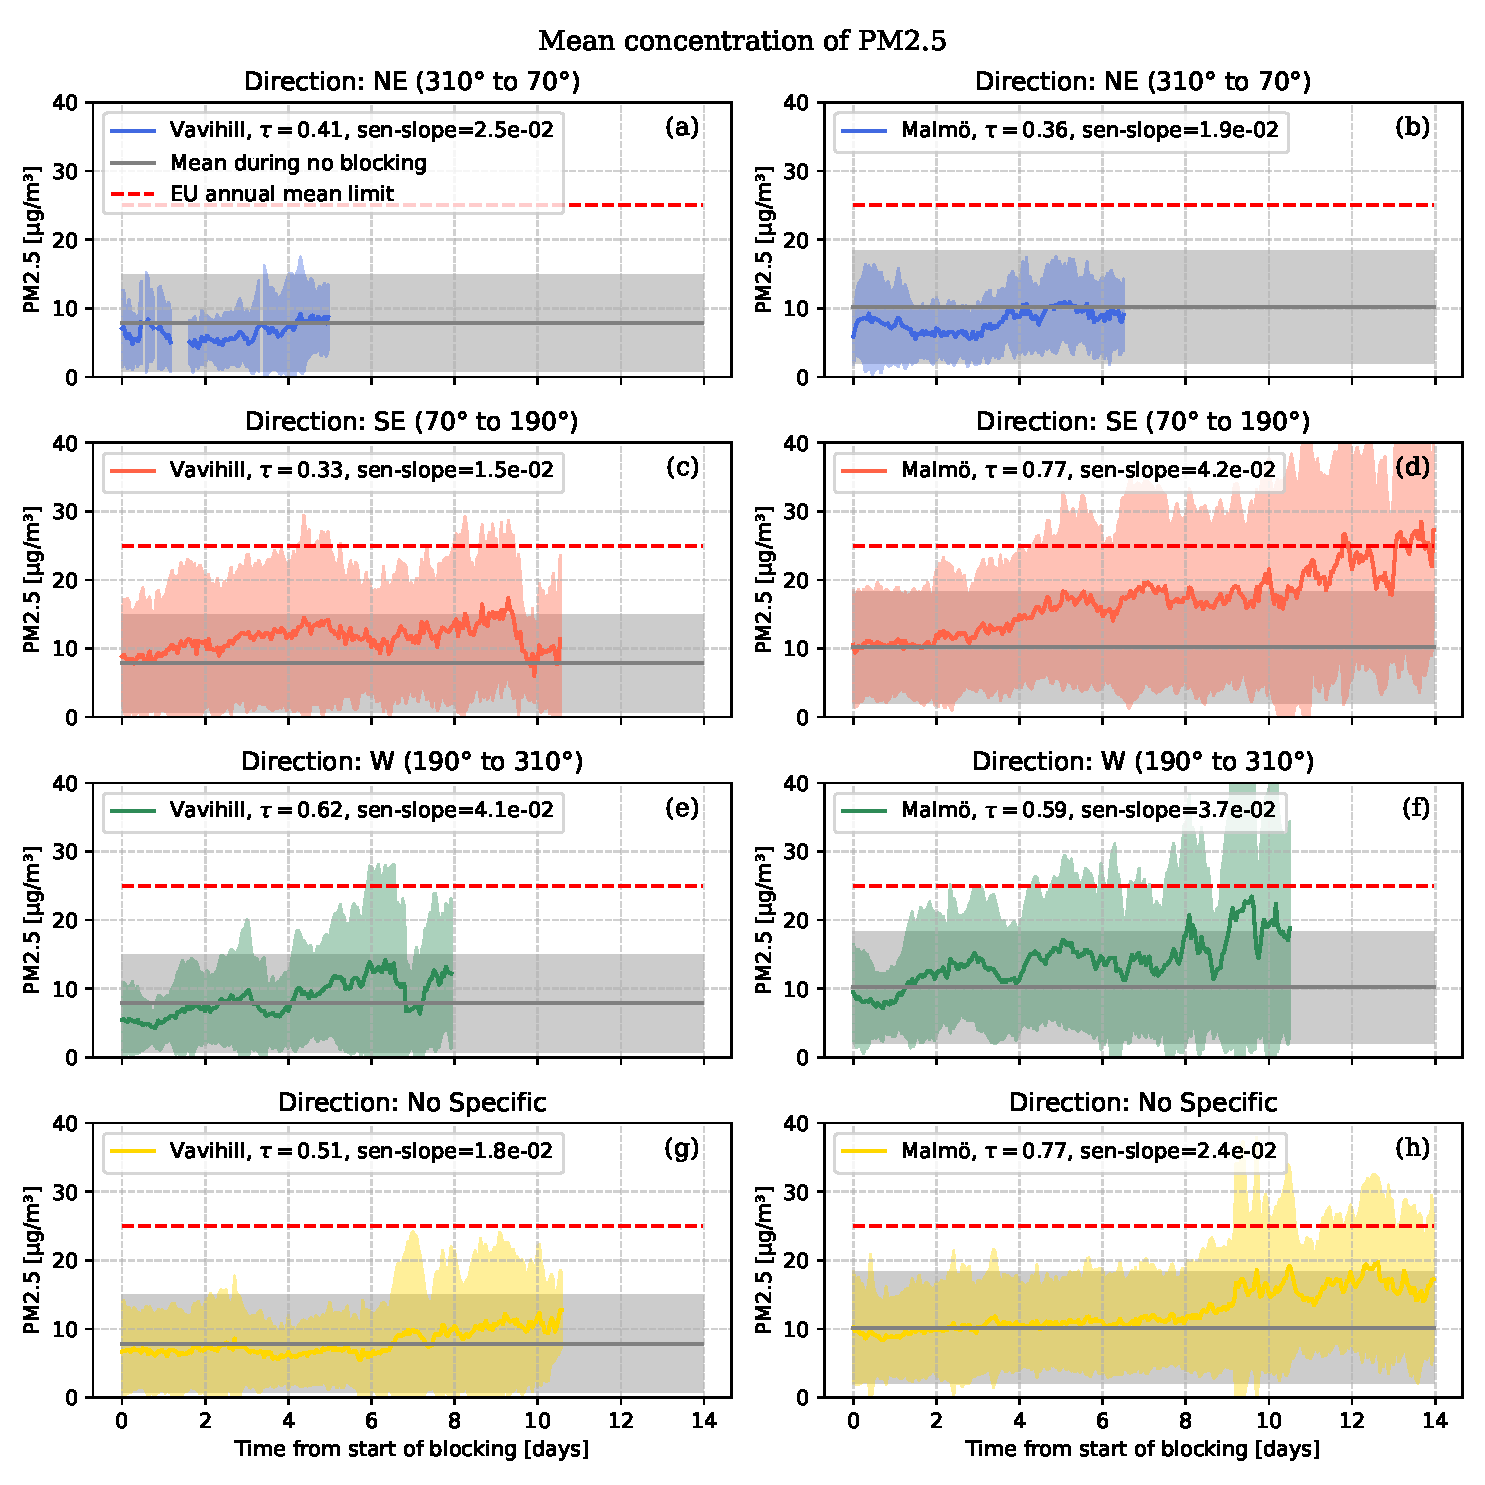
\includegraphics[width=\textwidth]{Figures/Meanplot_dir.pdf}
    \caption{These plots show how \PM concentrations in Vavihill and Malmö evolve for different wind directions. A minimum number of blocking events was still put to eight, resulting in some directions having very little data.}
    \label{fig:Meanplot_wind}
\end{figure}

 

\subsection{The change in aerosol concentrations depending on season}
The seasonal change in concentrations of \PM can be seen in \autoref{fig:Meanplot_seasonal}. From these plots, it is clear that the concentration during the summer for both Vavihill and Malmö does not indicate an increase nor high levels of \PM. In the case of Vavihill 22.9\% of the blocking events occurred during the winter, 27.6\% during the spring, 24.2\% during the summer and 26.7\% during the autumn. In the case of Malmö, 22.0\% of the blocking events occurred during the winter, 32.7\% during the spring, 18.0\% during the summer and 27.4\% during the autumn.

A slight increase can be seen in the case of spring for both locations \autoref{fig:Meanplot_seasonal} (c) and (d). A larger increase can be seen during the autumn, where high levels of \PM  can be observed towards the end of the period. The winter in Vavihill indicates an increase in the \PM  concentrations, although the standard deviation indicates highly dispersed data. Although the $\tau$-value during the winter in Malmö is relatively low, Sen's slope indicate a stronger increase. From the graph one can see an increase in \PM  concentrations, although the levels seem to decrease towards the end of the period. 

\begin{figure}[H]
    \centering
    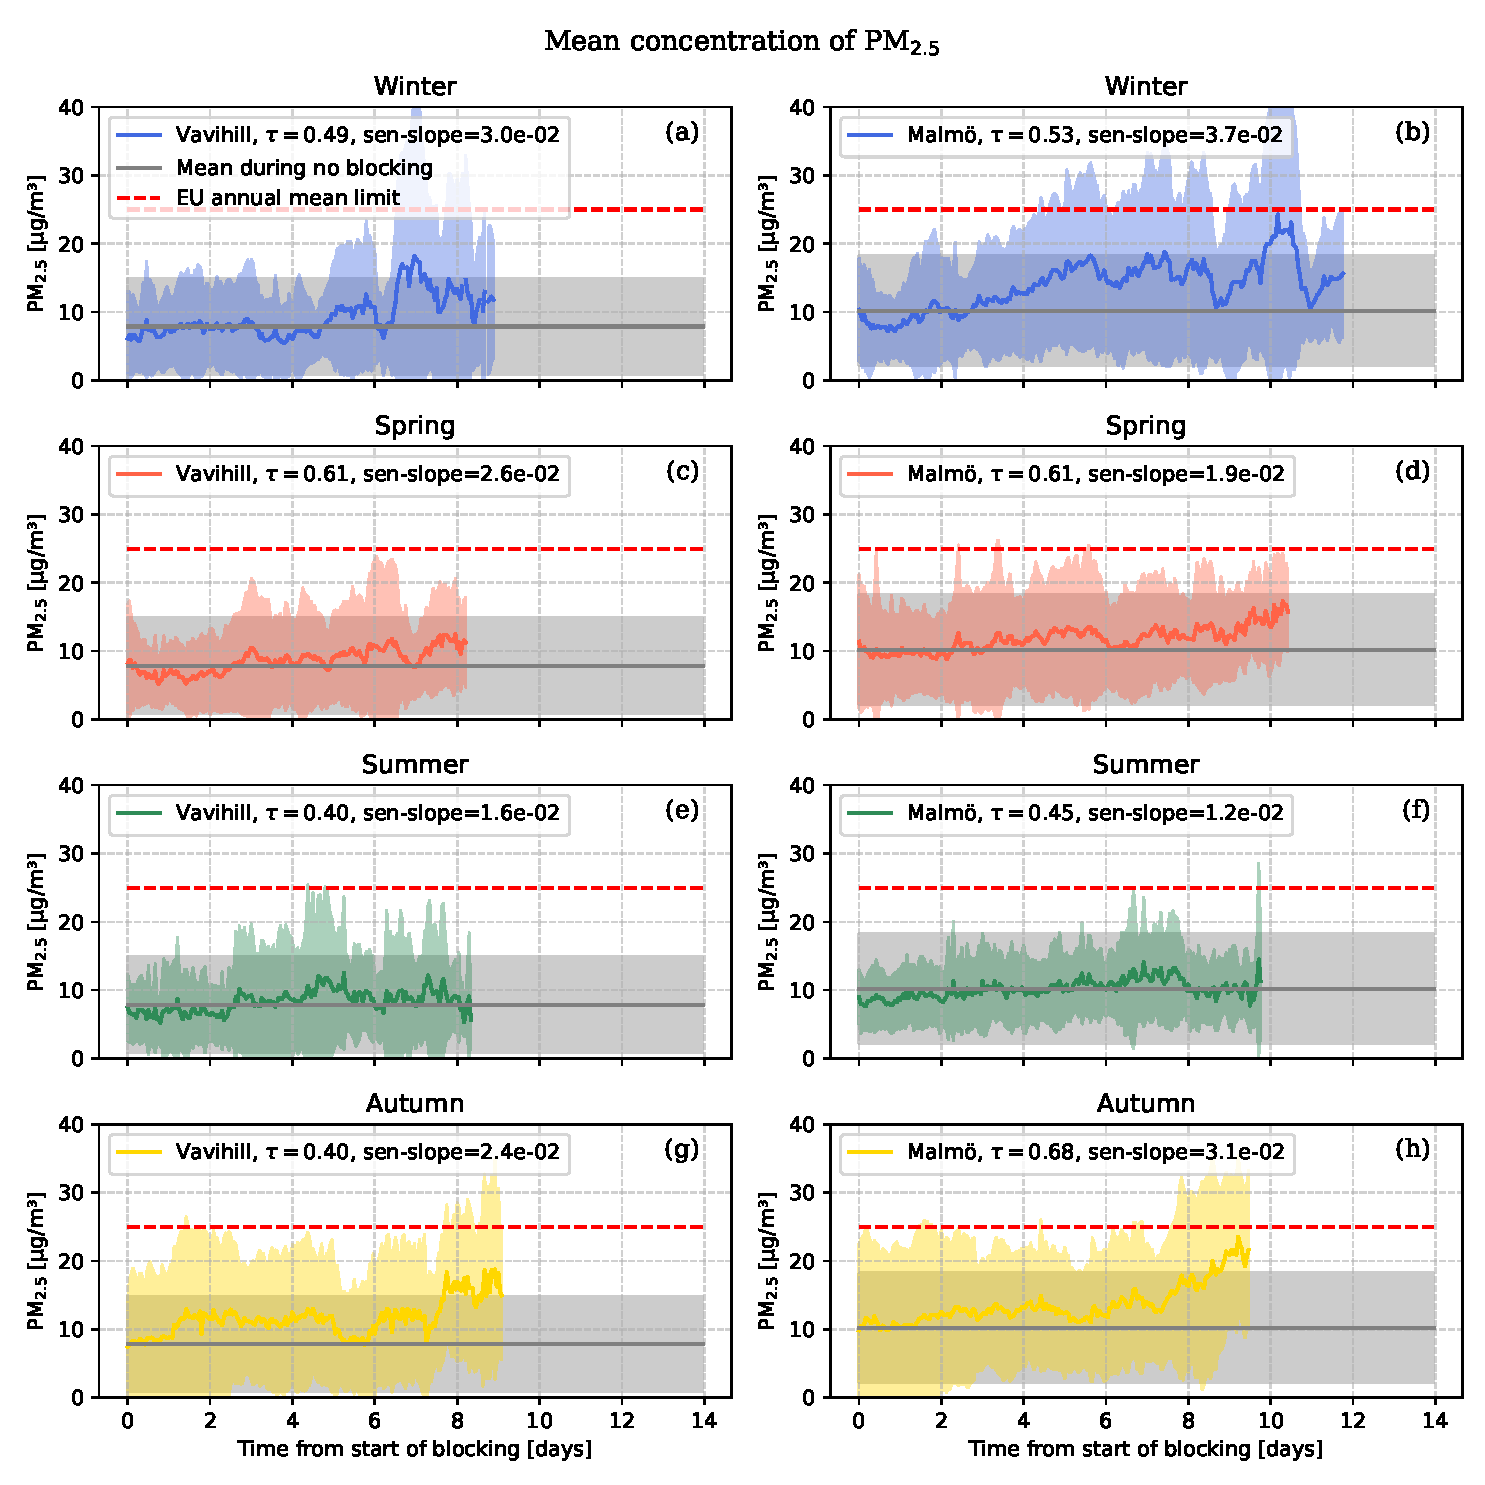
\includegraphics[width=\textwidth]{Figures/Meanplot_seasonal.pdf}
    \caption{These plots show \PM concentrations in Vavihill and Malmö for different seasons. }
    \label{fig:Meanplot_seasonal}
\end{figure}
 

\subsection{The evolution of \texorpdfstring{\PM }{PM2.5} depending on pressure strength}
The increase in \PM  concentrations depending on the strength of the high-pressure blocking event can be seen in \autoref{fig:Meanplot_pressure}. In the case of Vavihill, 20.3\% of the blocking events occurred with a mean pressure below 1020 hPa 45.5\% occurred between 1020 and 1025 hPa and 34.3\% occurred with a mean pressure over 1025hPa. In the cas of Malmö, it is important to note that 16.2\% of the blocking events occurred with a mean pressure below 1020 hPa 48.2\% occurred between 1020 and 1025 hPa and 35.6\% occurred with a mean pressure over 1025hPa.

From the plots, we can observe similar behaviour in the two locations. In the case of weaker high-pressure blocking events no clear monotonic increase nor highly elevated levels of \PM can be seen, as seen in (a) and (b). In the case of medium strong high-pressure blocking events we see a stronger increase in the case of Vavihill $\tau$=0.60 and weaker in Malmö from $\tau$=0.30. However when observing both plots one can see an increase for both plots around day nine, as seen in (c) and (e). In the case of stronger high-pressure blocking events we see a strong increase in the case for Malmö, and not as clear increase in the case of Vavihill. However when viewing the plots one can observe that the levels of \PM in the case of Vavihill exceed the normal range towards the end of the period. In the case of Malmö we can see a very strong increase towards the ned, where we reach the EU annal mean limit. 

\begin{figure}[H]
    \centering
    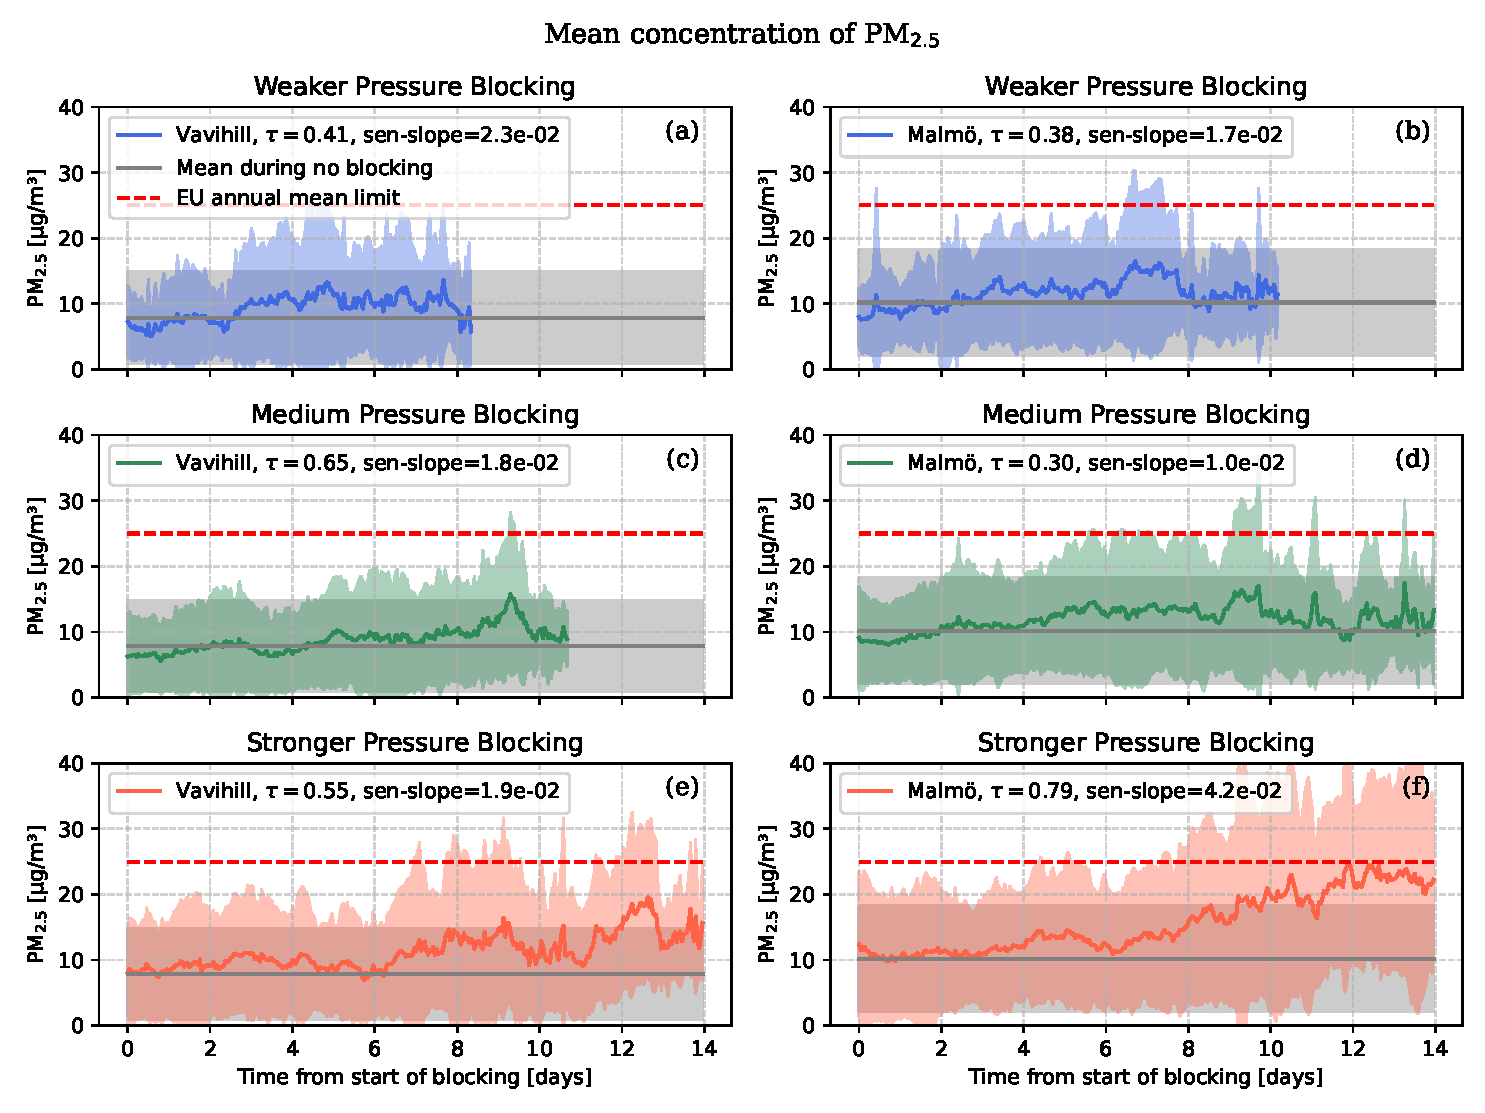
\includegraphics[width=\textwidth]{Figures/Meanplot_pressure.pdf}
    \caption{These plots show \PM concentrations in Vavihill and Malmö for different pressure strengths for high-pressure blocking events.}
    \label{fig:Meanplot_pressure}
\end{figure}


From the plots above, it is clear that the high elevations of \PM  occur after nine to 13 days. This is an interesting result since this indicates that prolonged periods of high-pressure blocking events indicate an accumulative increase of \PM, which can be seen in \autoref{fig:Meanplot_Comparison} where we see that the combination of all the other plots resulted in a steady increase in the case of Malmö, and an increase in the case of Vavihill. The only cases where we do not see this are in the case of medium strong high-pressure blocking events. The result of weaker high-pressure blocking events is more difficult to analyse since we do not have any result for days after day nine. However, no significant increase is observed leading up to this point, indicating an absence of further increase after this point. This result points towards the fact that for stronger high-pressure blocking events, we observe an increase in the concentration of \PM  after nine to thirteen days regardless of the type of high-pressure blocking event, even though different types of high-pressure blocking events may differ in the increase.

\subsection{The frequency of high pressure blocking events}
The last task was to determine whether high-pressure blocking events have become more common. When looking at the number of high-pressure blocking events per year, no significant change in frequency could be seen (see \autoref{fig:number_of_blockings}). Since the highest levels of \PM  occurred toward the end of the events (see \autoref{fig:Meanplot_Comparison}, \autoref{fig:Meanplot_wind}, \autoref{fig:Meanplot_seasonal}, and \autoref{fig:Meanplot_pressure}), the frequency of longer high-pressure blocking events was also examined. However, no increase could be observed in any of the cases. More interestingly a small decrease can be observed from the $\tau$-values and the Sen's slope values. However one must note that the p-values are much larger here than before, indicating towards a more random system. 

\begin{figure}[H]
    \centering
    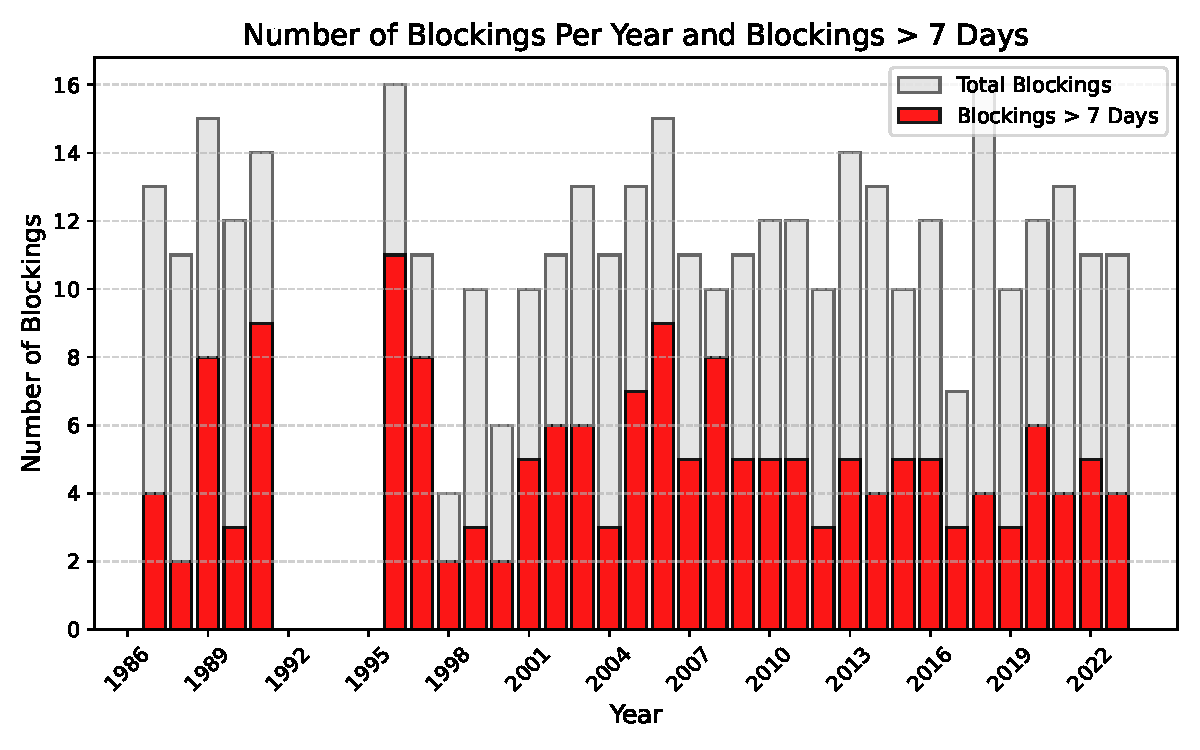
\includegraphics[width=0.7\textwidth]{Figures/BlockingsPerYear.pdf}
    \caption{fig: This plots shows the change in frequency of high-pressure blocking events. The plots also indicates the change in events longer than seven and ten days. }
    \label{fig:number_of_blockings}
\end{figure}

In \autoref{fig:Number_of_Blocking_Days_Per_Year}, the number of days under high-pressure blocking events per year can be seen. Here, the total, seasonal, and pressure strength dependence can be observed. The reason for not including the directional dependence is that no wind data was available for this period. the number of days under high-pressure blocking events. Even here a slight increase can be seen in most plots, especially the total blocking days per year (h). 


\begin{figure}[H]
    \centering
    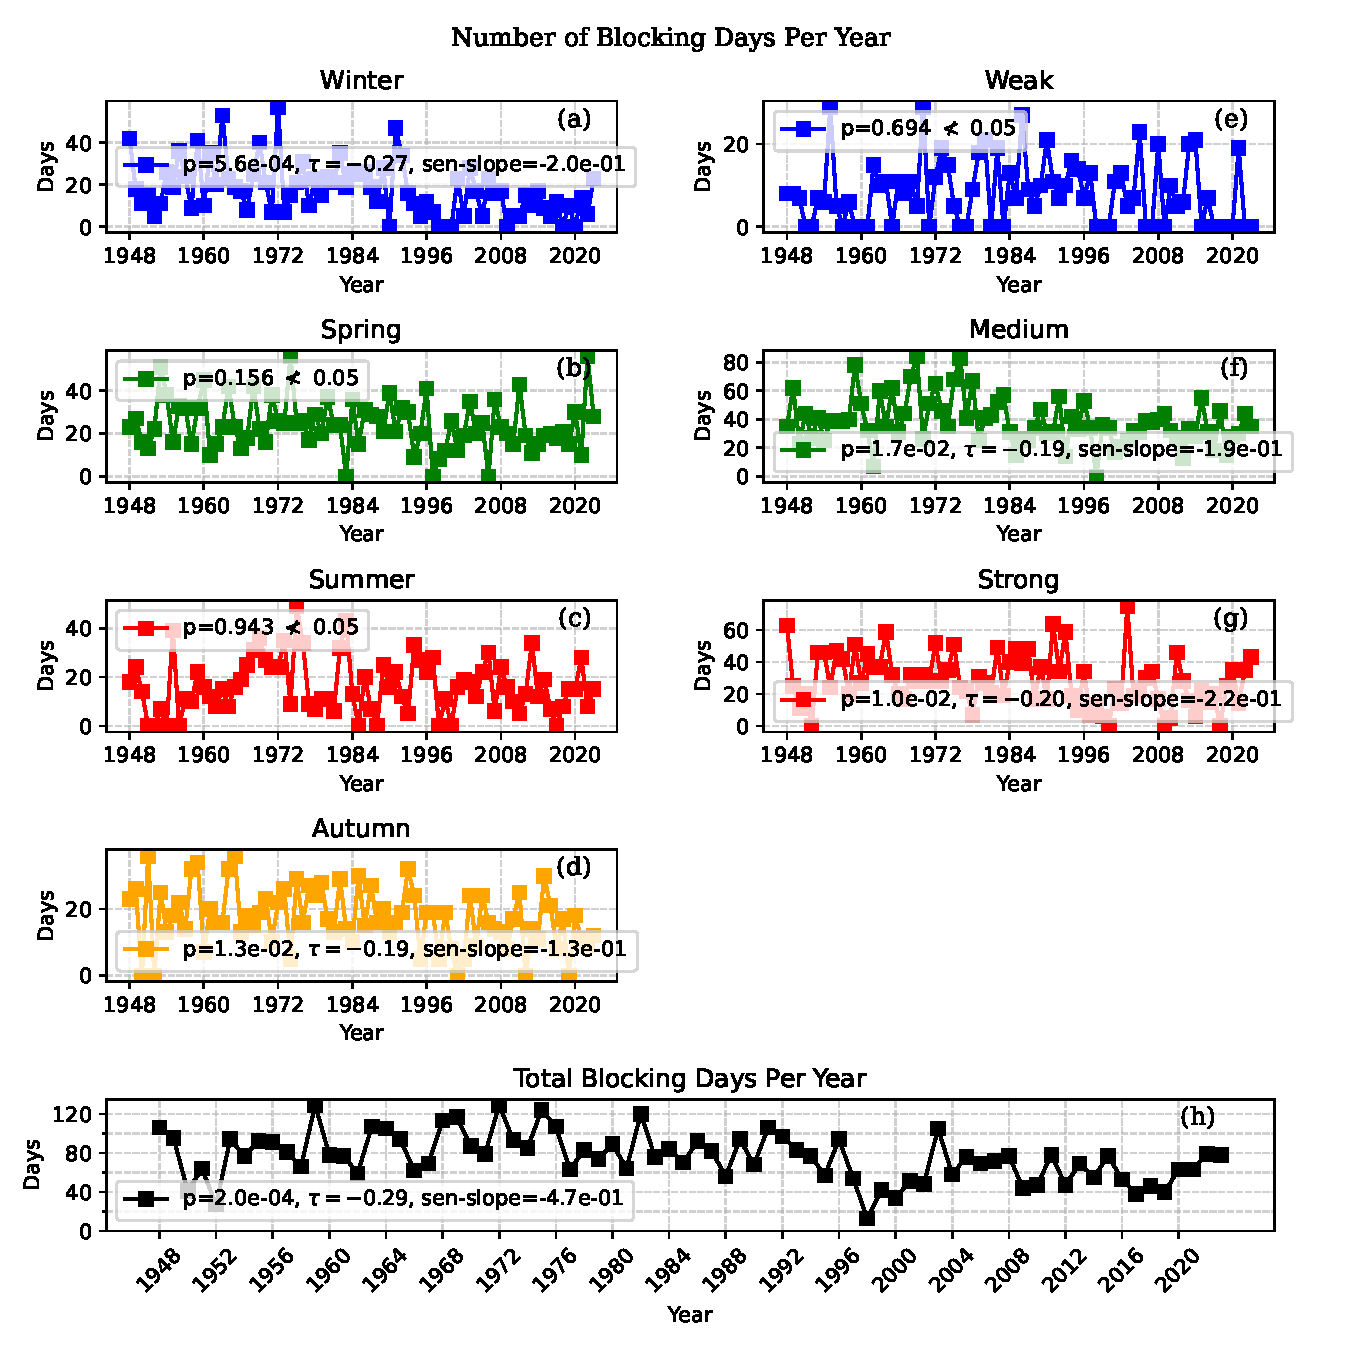
\includegraphics[width=\textwidth]{Figures/blocking_days_per_year_all.pdf}
    \caption{These plots show the change in frequency of days under high-pressure blocking events. The number of days under a high-pressure blocking event each year, during each season, and for different pressure strengths can also be seen.}
    \label{fig:Number_of_Blocking_Days_Per_Year}
\end{figure}

When observing slight decline of the frequency of the hig-pressure blocking events in \autoref{fig:number_of_blockings} and \autoref{fig:Number_of_Blocking_Days_Per_Year} one must note that the low $\tau$-values indicate that the trend is not monotonic. Furthermore, the large p-values indicate that the trend is not as non-random as seen in in the mean aerosol concentration plots observed in Figures~\ref{fig:Meanplot_Comparison}--\ref{fig:Meanplot_pressure}. This indicates that this trend is more likely caused to randomness, and should not be seen as a result. However, one can do the observation that the no type of high-pressure blocking event has become more common during the last 74 years. 
